\documentclass[titlepage=firstcover, captions=tableheading]{scrartcl}
\usepackage{microtype}
\usepackage{amsmath}
\usepackage{polyglossia}
\usepackage{graphicx}
\usepackage{booktabs}
\usepackage{siunitx}
\usepackage{hyperref}
\usepackage{caption}
\usepackage{float}
\setdefaultlanguage{german}
\title{V354 Gekoppelte und erzwungene Schwingungen}
\author{
Connor Magnus Böckmann \\ email: \href{mailto:connormagnus.boeckmann@tu-dortmund.de}{connormagnus.boeckmann@tu-dortmund.de}
\and Tim Theissel \\ email: \href{mailto:tim.theissel@tu-dortmund.de}{tim.theissel@tu-dortmund.de}}
\begin{document}
\maketitle
\newpage
\tableofcontents
\newpage
\section{Zielsetzung}
Das Ziel des Versuchs ist die Untersuchung eines RCL-Schwingkreises. Dabei soll der reale gedämpfte Schwingkreis anhand der Zeitabhängigkeit der Amplituden, des effektiven Widerstandes, dem aperiodischen Grenzfall und die Frequenzabhängigkeiten der Kondensatorspannung und ihrer Phase zur Erregerspannung. 
\section{Theoretische Grundlagen}
Beim in diesem Versuch untersuchten Schwingkreis handelkt es sich um einen RCL-Schwingkreis. Dieser enthält, verglichen mit dem RC-Kreis, neben dem Kondensator und dem Widerstand noch eine Spule mit Induktivität L. Dadurch ergibt sich ein zweiter Energiespeicher in Form der Spule. Diese ermöglicht ein Pendeln der Energie zwischen den beiden Energiespeichern, Spule und Kondensator. Das RCL-System schwingt also periodisch hin und her. Ohne Energieverbraucher, zum Beispiel den Widerstand, würde das System unendlich lange ungedämpft schwingen. Da der Widerstand aber elektrische Energie in Wärme umwandelt, geht darüber Energie verloren und der Schwingkreis wird gedämpft. Besonders von Interesse ist dabei das Zeitgesetz.
\subsection{Differentialgleichung für eine gedämpfte Schwingung-Herleitung und Lösung}
Vereinfacht lässt sich der RCl-Schwingkreis darstellen wie in Abb. 1. Daraus lässt sich erkennen, dass die zweite Kirchhoffsche Regel hier verwendet werden kann.
\begin{figure}[H]
    \centering
    \includegraphics{"Schaltkreis_RCL.png"}
    \caption{RCL-Schwingkreis}
\end{figure}
Mit der zweiten Kirchhoffschen Regel lässt sich die Spannung im System darstellen:
\begin{align}
    U_R(t)+U_C(t)+U_L(t)&=0\nonumber\\
    U_R(t)&=R\cdot I(t)\nonumber\\
    U_C(t)&=\frac{Q(t)}{C} \text{ (Q(t)=Ladung des Kondensators)}\nonumber\\
    U_L(t)&=L\frac{dI}{dt} \text{ (Induktionsgesetz)}\nonumber\\\nonumber
\end{align}
Es folgt also daraus:
\begin{equation}
  L\frac{dI}{dt}+RI+Q\frac{Q}{C}=0  \nonumber
\end{equation}
Die gesuchte Schwingungsgleichung ergibt sich dann mit 
\begin{equation}
    I=\frac{dQ}{dt}\nonumber
\end{equation}
aus der ersten Ableitung zu 
\begin{equation} \label{DGL}
    \frac{d^2I}{dt^2}+\frac{RdI}{Ldt}+\frac{I}{LC}=0
\end{equation}
Geloest wird diese lineare, homogene DGL mit dem Ansatz 
\begin{equation}
    \tau(t)=\xi e^{j\omega t}\nonumber
\end{equation}
Dabei sind \xi und \omega komplexe Zahlen und $j=\sqrt{-1}$.
Daraus erhaelt man 
\begin{equation}
    (-\omega^2+j\frac{R}{L}\omega+\frac{1}{LC})\xi e^{j\omega t} \nonumber
\end{equation}
Die DGL wird nun fuer beliebige \xi und beliebige t erfuellt, solange \omega die charakteristische Gleichung 
\begin{equation}
    \omega^2-j\frac{R\omega}{L}-\frac{1}{LC}=0 \nonumber
\end{equation}
Daher muss \omega einen der beiden Werte 
\begin{equation}
    \omega=j\frac{R}{2L}\pm \sqrt{\frac{1}{LC}-\frac{R^2}{4L^2}}\nonumber
\end{equation}
Alle Loesungen der DGL lassen sich dann ausdruecken als 
\begin{equation}
    \tau=\xi_1e^{j\omega_1t}+\xi_2e^{j\omega_2t}\nonumber
\end{equation}
Ausserdem werden die Abkuerzungen 
\begin{align}\label{Reff}
    2\pi\mu:&=\frac{R}{2L}\\
    2\pi v:&=\sqrt{\frac{1}{LC}-\frac{R^2}{4L^2}}\nonumber\\
\end{align}
$\tau(t)$ laest sich dann schreiben als
\begin{equation}\label{Klammer}
    \tau(t)=e^{-2\pi\mu t}(\xi_1e^{j2\pi vt}+\xi_2e^{-j2\pi vt})
\end{equation}
Die Loesung haengt nun massgebend davon ab, ob $\frac{1}{LC}$ groesser oder kleiner als $\frac{R^2}{4L^2}$. Dieser Umstand entscheide nun, ob v reell oder imaginaer ist. Daher ist eine Fallunterscheidung notwendig.
\subsection{1. Fall: $\frac{1}{LC}>\frac{R^2}{4L^2}$}
Unter diesen Bedingungen ist dann $\xi_1 =\bar{\xi_2}$, damit die Loesung $\tau(t)$ reell wird.
Das laesst sich ausdruecken durch den Ansatz
\begin{align}
    \xi_1&=\frac{1}{2}A_0e^{j\eta}\nonumber\\
    \xi_2&=\frac{1}{2}A_0e^{-j\eta}\nonumber
\end{align}
Fuer $\tau(t)$ unter Benutzung der Euler-Identitaet gilt
\begin{equation}
    \frac{e^{j\varphi}+e^{-j\varphi}}{2}=\cos\varphi \nonumber
\end{equation}
Daher ergibt sich fuer den geklammerten Ausdruck aus \ref{Klammer} eine reine oszillatorische Funktion.
\begin{equation}\label{Reff2}
    I(t)=A_0e^{-2\pi\mu t}\cos(2\pi vt+\eta)\nonumber
\end{equation}
Diese Gleichung stellt eine gedaempfte Schwingung dar. Die Schwingung ist also harmonisch, geht aber mit fortschreitender Zeit exponentiell gegen null. Die Schwingungsdauer laesst sich dabei ausdruecken als:
\begin{equation}
    T=\frac{1}{v}=\frac{2\pi}{\sqrt{\frac{1}{LC}-\frac{R^2}{4L^2}}}\nonumber
\end{equation}
Sie naehert sich dem Wert
\begin{equation}
    T_0=\frac{2\pi}{\omega_0}=2\pi\sqrt{LC}\nonumber
\end{equation}
der ungedaempften Schwingung an, wenn $\frac{R^2}{4L^2}$ klein gegen $\frac{1}{LC}$.
Die Amplitudenabnahmmegeschwindigkeit wird charakterisiert durch $2\pi\mu=\frac{R}{2L}$.
Die Amplitude geht dabei nach der Zeit 
\begin{equation}\label{Tex}
    T_{ex}=\frac{1}{2\pi\mu}=2\pi\sqrt{LC}
\end{equation}
auf den e-ten Teil des Startwerts zurueck. $T_ex$ wird Abklingdauer genannt.
\subsection{2. Fall: Aperiodische Daempfung fuer $\frac{1}{LC}<\frac{R^2}{4L^2}$}
Die Loesung I(t) enthaelt fuer diesen Fall keinen oszillatorischen Anteil mehr. Dieser Fall nennt sich aperiodische Daempfung. Von besonderer Bedeutung ist der Spezialfall des aperiodischen Grenzfalls.
\begin{equation}\label{Rap}
    \frac{1}{LC}=\frac{R_ap^2}{4L^2}
\end{equation}
Dadurch ist $v=0$ und $I(t)=Ae^{-\frac{Rt}{2L}}=Ae^{-\frac{t}{\sqrt{LC}}}$
Der aperiodische Grenzfall stellt einen Fall ohne Ueberschwingen dar fuer den die Schwingung am schnellsten gegen null geht.
\subsection{Differentialgleichung fuer erzwungene Schwingungen}
Im Folgenden wird das schwingfaehige System durch eine aeussere, periodische Kraft ausgelenkt. Im Fall des RCL-Schwingkreises handelt es sich dabei um eine sinusfoermige Wechselspannung u(t).
\begin{equation}
    u(t)=U_0e^{j\omega t}\nonumber
\end{equation}
Die in den vorigen Abschnitten beschriebene Differentialgleichung \ref{DGL} nimmt hier somit die Form
\begin{equation}
    L\frac{d\xi}{dt}+R\xi+\frac{Q}{C}=U_0e^{j\omega t}\nonumber
\end{equation}
oder 
\begin{equation}\label{DGL 2}
    LC\frac{d^2u_C}{dt^2}+RC\frac{du_C}{dt}+u_C=U_0e^{j\omega t}
\end{equation}
an. 
Q(t) stellt hierbei die Ladung auf dem Kondensator dar, weshalb damit die Spannung folgende ist:
\begin{equation}
    u_C(t)=\frac{Q(t)}{C}\nonumber
\end{equation}
Betrachtet wird im Folgenden vorallem die Amplitude der Kondensatorspannung $u_C(t)$ mit ihrem Phasenunterschied gegenueber der Erregerspannung u(t). Besonderes Augenmerk wird dabei auf ihre Frequenzabhaengigkeit gelegt.\\
Der Ansatz ist
\begin{equation}\label{Ansatz}
    u_C(\omega, t)=\xi(\omega)e^{j\omega t} (\xi komplex) 
\end{equation}
Nun wird \ref{Ansatz} in \ref{DGL 2} eingesetzt und die Bestimmungsgleichung $-LC\omega^2\xi+j\omega RC\xi+\xi=U_0$ nach \xi  aufgeloest.
\begin{equation}
    \xi=\frac{U_0}{1-LC\omega^2+j\omega RC}=\frac{U_0(1-LC\omega^2-j\omega RC)}{(1-LC\omega^2)^2+\omega^2R^2C^2} \nonumber
\end{equation}
Der Betrag betraegt dann 
\begin{equation}\label{Betrag}
    |\xi|=\sqrt{Re^2(\xi)+Im^2(\xi)}=U_0\sqrt{\frac{(1-LC\omega^2)^2+\omega^2R^2C^2}{((1-LC\omega^2)^2)+\omega^2R^2C^2)^2}}
\end{equation}
mit der Phase
\begin{equation}
    \tan \varphi(\omega)=\frac{Im(\xi)}{Re(\xi)}=\frac{-\omega RC}{1-LC\omega^2}\nonumber
\end{equation}
beziehungsweise
\begin{equation}\label{phi}
    \varphi(\omega)=\arctan(\frac{-\omega RC}{1-LC\omega^2})
\end{equation}
Der Betrag der Loesungsfunktion nach \ref{Ansatz} entspricht dabei dem Betrag von \xi. Somit erhaelt man aus \ref{Betrag} als Ergebnis
\begin{equation} \label{Resonanzkurve}
    U_C(\omega)=\frac{U_0}{\sqrt{(1-LC\omega^2)^2+\omega^2R^2C^2}}
\end{equation}
Durch diese Beziehung laesst sich also nun die gesuchte Frequenzabhaengigkeit zwischen der Kondensatorspannung und der Frequenz $\omega$. Dieser Zusammenhang nennt sich Resonanzkurve. Fuer $\omega\rightarrow\infty$ geht $U_C\rightarrow 0$ und fuer $\omega\rightarrow 0$ geht $U_C\rightarrow U_0$. Bei einer bestimmten Frequenz gibt es ein $U_C$, welches groesser als die urspruengliche Erregeramplitude $U_0$ ist. Diese Frequenz nennt sich Resonanzfrequenz und das zugehoerige Phaenomen nennt sich Resonanz. Gegeben wird die Resonanzfrequenz durch
\begin{equation}
    \omega_{res}=\sqrt{\frac{1}{LC}-\frac{R^2}{2L^2}} 
\end{equation}
Besonderer Betrachtung wird der Fall der schwachen Daempfung, also $\frac{R^2}{2L^2}<<\frac{1}{LC}$, unterzogen. Dort naehert sich die Resonanzfrequenz naemlich der Kreisfrequenz des ungedaempften Schwingkreises an. Die Kondensatorspannung uebertrift die Erregerspannung um den Faktor $\frac{1}{\omega_0RC}$, die so genannte Resonanzueberhoehung oder Guete q eines Schwingkreises.
\begin{equation}\label{Umax}
    U_{c,max}=\frac{1}{\omega_0RC}U_0=\frac{1}{R}\sqrt{\frac{L}{C}}U_0 
\end{equation}
Es laesst sich bereits erkennen, dass die Kondensatorspannung fuer $R\rightarrow 0$ gegen $\infty$ geht. Es handelt sich dabei um die so genannte Resonanzkatastrophe. Ausserdem ist die Breite der Resonanzkurve in \ref{Resonanzkurve} ein Mass fuer die Schaerfe eines Schwingkreises. Charakterisiert wird sie durch die Frequenzen bei denen $U_C$ auf den $\frac{1}{\sqrt{2}}$-sten Bruchteil seines Maximums \ref{Umax} abgefallen ist. Diese werden $\omega_+$ und $\omega_-$ genannt und werden durch 
\begin{equation}
    U_{c,max}=\frac{1}{\omega_0RC}U_0=\frac{1}{R}\sqrt{\frac{L}{C}}U_0 \nonumber
\end{equation}
gegeben. Unter Beachtung, dass $\frac{R^2}{L^2}<<\omega_0^2$ ist, folgt fuer die Breite der Resonanzkurve
\begin{equation}
    \omega_+-\omega_-\approx \frac{R}{L}\nonumber
\end{equation}
Somit besteht zwischen der Guete q und der Breite der Resonanzkurve die folgende Beziehung:
\begin{equation}
    q=\frac{\omega_0}{\omega_+-\omega_-}\nonumber
\end{equation}
Das Verhalten aendert sich fuer starke Daempfung, also $\frac{R^2}{2L^2}>>\frac{1}{LC}$, grundlegend. Es existiert keine Frequenzueberhoehung mehr. Stattdessen geht $U_C$ von $U_0$ aus mit wachsender Frequenz monoton gegen 0. Bei hinreichend hohen Frequenzen faellt $U_C$ proportional zu $\frac{1}{\omega^2}$.\\
Im Folgenden soll ausserdem noch die Frequenzabhaengigkeit der Phase zwischen Erreger- und Kondensatorspannung untersucht werden. Nach dem Ansatz aus \ref{Ansatz} gibt Gleichung \ref{phi} den Zusammenhang zwischen $\varphi$ und $\omega$ wieder. Gleichung \ref{phi} sagt dabei aus, dass bei kleinen Frequenzen Kondensator- und Erregerspannung praktisch in Phase sind. Im Gegensatz dazu verschiebt sich die Kondensatorspannung bei sehr grossen Frequenzen um $\pi$ und hinkt dadurch der Erregerspannung hinterher. 
\subsection{Impedanz eines Schwingkreises}
Ein RCL-Serienschwingkreis kann auch als ein Zweipol aufgefasst werden. 
\begin{figure}[H]
    \centering
    \includegraphics{"Schaltkreis_RCL.png"}
    \caption{Serienschwingkreis als Zweipol}
\end{figure}
An den Enden des Zweipols laesst sich ein Widerstand feststellen. Dieser ist frequenzabhaengig und wird Impedanz. Sie wird auf Grund der haeufig vorhandenen Phasenverschiebung zwischen Strom und Spannung als komplexe Zahl definiert.
\begin{equation}
    z=x+iy \nonumber
\end{equation}
Dabei sind x und y reelle Widerstaende. Sie werden Blindwiderstand (Reaktanz) und Wirkwiderstand genannt. Der Betrag der Impedanz 
\begin{equation}
    |z|=\sqrt{x^2+y^2} \nonumber
\end{equation}
nennt sich Scheinwiderstand. Die Darstellung der Impedanz $z(\omega)$ in der komplexen Zahlenebene wird Ortskurve genannt und laesst sich duch einen Vektor aus dem Ursprung darstellen. Die Laenge des Vektors entspricht dem Scheinwiderstand. Der Winkel $\alpha$ zwischen dem Vektor und der reellen Achse ist genauso gross wie die Phasenverschiebung zwischen Spannung und Strom im Serienschwingkreis als Zweipol.
\begin{figure}[H]
    \centering
    \includegraphics[width=0.45\textwidth]{"RCL_Serienschwingkreis_komplex.png"}
    \caption{Darstellung der Impedanz des Serienschwingkreises als Zweipol in der komplexen Zahlenebene}
\end{figure}
Die Impedanz z errechnet sich nun folgendermassen mit den Widerstandsoperatoren
\begin{align}
    z_C&=-i\frac{1}{C\omega} \text{ (Widerstand der Kapazitaet)} \nonumber \\
    z_L&=iL\omega \text{ (Widerstand der Induktivitaet)}\nonumber \\
    z_R&=R_S \text{ (ohmscher Widerstand)} \nonumber\\
\end{align}
zu 
\begin{equation}
    z_S=R_S+i(L\omega-\frac{1}{C\omega}) \nonumber
\end{equation}
$x_S$ und $y_S$ sind dann
\begin{align}
    x_S&=R_S \nonumber \\
    y_S&=iL\omega-\frac{1}{C\omega} \nonumber \\
    |z_S|&=\sqrt{R_S^2+(L\omega-\frac{1}{C\omega})^2} \label{Scheinwiderstand}
\end{align}
Die Frequenzunabhaengigkeit von $x_S$ sorgt fuer eine Ortskurve, welche immer parallel zur imaginaeren Achse verlaeuft und an der Stelle $R_S$ die reelle Achse schneidet. Der Scheinwiderstand erreicht auf Grund von \ref{Scheinwiderstand} an der Stelle $\omega=\omega_0=\frac{1}{\sqrt{LC}}$ sein Minimum $R_S$. Fuer $\omega\rightarrow 0$ und $\omega\rightarrow\infty$ geht der Widerstand gegen $\infty$. 
\subsection{Parallelschwingkreis als Zweipol}
\begin{figure}[H]
    \centering
    \includegraphics[width=0.45\textwidth]{"RCL_Parallelschwingkreis.png"}
    \caption{Parallelschwingkreis als Zweipol}
\end{figure}
\noindent Die Impedanz eines Parallelschwingkreises soll der Vollstaendigkeit halber auch noch kurz erwaeht werden. Diese errechnet sich dann zu
\begin{equation}\label{Impedanz_parallel}
    z_p=\frac{\frac{1}{R_p}+i(\frac{1}{\omega L}-C\omega)}{\frac{1}{R_p^2}+(\frac{1}{L\omega}-C\omega)^2} 
\end{equation}
und der Scheinwiderstand dementsprechend zu
\begin{equation}
    |z_p|=\frac{1}{\sqrt{\frac{1}{R_p^2}+(\frac{1}{L\omega}-C\omega)^2}}
\end{equation}
$|z_p|$ durchlauft also nun bei $\omega_0=\frac{1}{\sqrt{LC}}$ ein Maximum mit dem Wert $R_p$. $|z_p|$ geht fuer $\omega\rightarrow 0$ gegen 0. Die Abhaengigkeit des Scheinwiderstandes von der Frequenz laesst sich wie folgt darstellen:
\begin{figure}[H]
    \centering
    \includegraphics[width=0.45\textwidth]{"RCL_Parallelschwingkreis_Abhaengigkeit.png"}
    \caption{Abhaengigkeit des Scheinwiderstandes von der Frequenz im Parallelschwingkreis}
\end{figure}
Aus \ref{Impedanz_parallel} ergibt sich fuer die Ortskurve des parallel geschalteten RCL-Schwingkreises ein Kreis mit dem Radius $\frac{1}{2}R_p$. Der Mittelpunkt ist dabei der Punkt $(0,\frac{1}{2}R_p)$, siehe ~\ref{fig:Parallel_Ortskurve}.
\begin{figure}[H]
    \centering
    \includegraphics[width=0.45\textwidth]{"RCL_Parallelschwingkreis_Ortskurve.png"} 
    \caption{Ortskurve eines Parallelschwingkreis}
    \label{fig:Parallel_Ortskurve}
\end{figure}

\section{Auswertung}

Zu Beginn dieser Auswertung ist zu sagen, dass sämtliche in dieser Auswertung vorkommenden Fehlerrechnungen mit der Python-Funktion "uncertainties" durchgeführt werden.


\noindent Durch die Bauteile werden bei diesem Versuch folgende Werte für den Schwingkreis vorgegeben:

\begin{align}
    L &= (16.78 \pm 0.09)µH  \nonumber  \\
    C &= (2.066 \pm 0.006)nF \nonumber \\
    R_1 &= (67.2 \pm 0.2) \Omega \nonumber \\
    R_2 &= (682 \pm 1) \Omega \nonumber
\end{align}

\subsection{Aufgabe 5a}

In diesem Aufgabenteil soll die Zeitabhängigkeit der Amplitude einer gedämpften Schwingung und daraus der Dämpfungswiderstand bestimmt werden.
Dafür wurden am Oszillograph die Amplituden abgelesen und dann gegen die Zeit in einem Diagramm dargestellt (\ref{5aD}).
Die abgelesenen Werte sind in Tabelle \ref{tab:5a} zu finden. 
Eine Ausgleichsrechnung mit einer Funktion der Form:
\begin{displaymath}
    b*e^{-2 * \pi * a * x}
\end{displaymath}

\noindent lifert den, in dem Diagramm \ref{5aD} zu sehenden, Graphen.
Diese Ausgleichsrechnung wurde mit der Python-Funktion "scipy.optimize" durchgeführt und liefert folgende Parameter für die Funktion:

\begin{center}
\begin{tabular}{ll @{${}\pm{}$}l}
    \toprule
    Parameter & Wert & Unsicherheit\\
    \midrule
    a & 0.001218 & 0.000017  \\
    b & 4.033851 & 0.035089  \\
\end{tabular}
\end{center}

\noindent Der Parameter a entspricht fast dem µ aus \ref{Reff2}.
Dadurch, dass die Zeitachse in diesem Diagramm die Einheit µs hat muss der Parameter a folgendermaßen angepasst werden.
Der Exponent der e Funktion aus \ref{Reff2} muss insgesamt einheitslos sein.
Da t allerdings die Einheit µs trägt muss a folglich den Kehrwert dieser Einheit tragen.
Deshalb müssten die beiden Parameter in SI-Einheitden wie folgt aussehen:
\begin{center}
    \begin{tabular}{ll @{${}\pm{}$}l}
        \toprule
        Parameter & Wert & Unsicherheit\\
        \midrule
        a & 1218 & 17  \\
        b & 4.033851 & 0.035089  \\
    \end{tabular}
    \end{center}
Mit diesem Parameter und den Beziehungen aus \ref{Reff}, 
lässt sich der effektive Dämpfungswiderstand bestimmen.
Nach dem Umstellung der Gleichung \ref{Reff} ergibt sich,
unter Verwendung des zu Begin der Auswertung vorgegebenen Wertes für L,
R\textsubscript{eff} zu:

\begin{displaymath}
    R_{eff} = 257 \pm 4 \Omega
\end{displaymath}

\noindent Es ist deutlich zu erkennen, dass der gegebene Wert für den eingebauten Widerstand überschritten wird.
Der gegebene Wert ist nämlich lediglich $R_1 = (67.2 \pm 0.2) \Omega$.
Der noch nicht betrachtete Generatorinnenwiderstand von 50 $\Omega$ verringert die Abweichung zwar etwas, 
allerdings ist diese immer noch sehr groß.
Dies könnte mit den verwendeten Geräten zusammenhängen. 
Die Werte für die Spannung müssen mit bloßem Auge vom Bildschirm des Oszillographen abgelesen werden.
Dabei enstehen Ablesefehler.
Eine weitere Fehlerquelle liegt bei der Eichung des Geräts. 
Die Funktion zur Eichung des Oszillographen sollte Das Gerät eine zur x-Achse parallele Linie anzeigen.
In der Realität war diese Linie Allerdings nicht parallel zur x-Achse. 
Dieser Umstand macht eine exakte Eichung sehr schwierig.
Es gibt auch noch den Fehler durch die Ungenauigkeit des berechneten Widerstands.
Diese fällt sehr klein aus, da nur Werte mit relativ geringen Fehlern in der REchnung verwendet werden.

\noindent Um nun die Abklingdauer T\textsubscript{ex} zu berechnen wird die Gleichung \ref{Tex} verwendet.
$a = 1218 \pm 17$

\begin{displaymath}
    T_{ex} = 0.0001307 \pm 0.0000018 s
\end{displaymath}

\begin{figure}[H]
    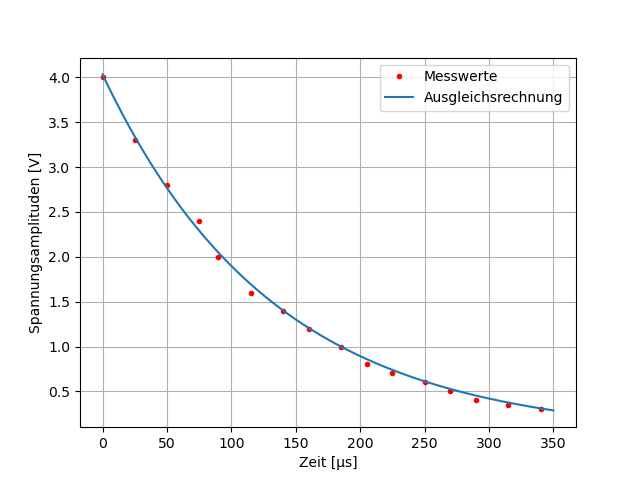
\includegraphics{5a.png}
    \caption{Spannungsamplituden-Diagramm}
    \label{5aD}
\end{figure}

\subsection{Aufgabe 5b}

Der germssene Wert R\textsubscript{ap} beträgt: 3250 $\Omega$.

\noindent Um R\textsubscript{ap} zu berechenen ist Formel \ref{Rap} zu verwenden.
Nach kurzen Umformungen lässt sich folgender Wert berechnen:
\begin{displaymath}
   R_{ap} = 5700 \pm 17 \Omega
\end{displaymath} 

\noindent Bei dieser Messung musste der Widerstand am Oszillographen, mit einem Drehrad, eingestellt und an diesem auch abgelesen werden.
Dabei gibt es schon kleinere Ablesefehler.
Das größere Problem ist hier allerdings, dass es im Auge des Betrachters liegt wann der aperiodische Grenzfall erreicht ist.
Der aperiodische Grenzfall lässt in seiner Definition zwar keine subjektive Interpretation zu, 
allerdings ist es auf dem Bildschirm des Oszillographen schwer zu erkennen, 
ob der aperiodische Grenzfall tatsächlich schon erreicht oder vielleicht sogar überschritten ist. 
Auch hier könnte die in Aufgabenteil 5a erwähnte Eichung ein großes Problem darstellen.

\subsection{Aufgabe 5c}

Die Resonanzüberhöhung lässt sich bestimmen,
indem in einem halblogarithmischen Diagramm U\textsubscript{C}/U gegen die Frequenz v aufgetragen wird.
Dabei wird die Resonanzüberhöhung als Peak des Graphen auftreten.

\noindent Das Diagramm sieht wie folgt aus:

\begin{figure}[H]
    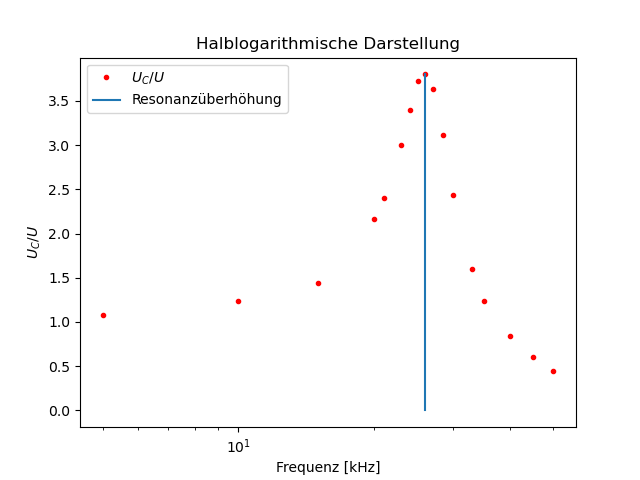
\includegraphics{5c.png}
    \caption{Resonanzüberhöhung}
    \label{5bD}
\end{figure}

\noindent Die Resonanzüberhöhung tritt bei einer Frequenz von 26kHz auf und beträgt q = 3,8.


\noindent Die Resonanzfrequenz lässt sich auch mit der Formel 

\begin{displaymath}
    q = \sqrt{\frac{L}{R^2C}} 
\end{displaymath}

\noindent berechnen.
\begin{displaymath}
   \omega_{res} 24.32\pm 0.08  kHz
\end{displaymath}

\noindent Die Abweichung der Resonanzüberhöhung vom theoretischen Wert liegt an den klassischen Fehlerquellen der graphischen Bestimmung von Werten.\\
Dazu gehören:\\
-Ablesefehler bei der Aufnahme von Messwerten die sich durch die Ausgleichsrechnung weiter fortpflanzen.\\
-Ungenauigkeiten der Ausgleichsrechnung.\\
-Eichfehler des Geräts.\\

\noindent Im folgenden Diagramm wird der Ausschnitt um die Resonanzfrequenz linear dargestellt.

\begin{figure}[H]
    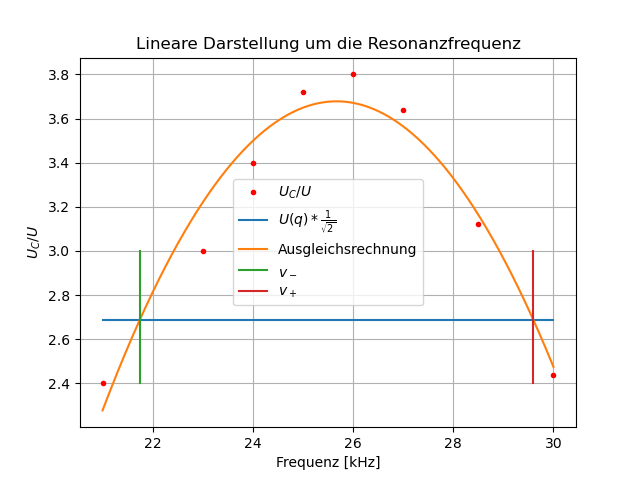
\includegraphics{5c2.png}
    \caption{Breite der Resonanzkurve}
    \label{5cD}
\end{figure}

\noindent Die Breite der Resonanzkurve ließ sich bestimmen, indem in diesem Bereich eine Ausgleichsrechnung mit einer Funktion der Form:

\begin{displaymath}
    a*(x-b)^2+c
\end{displaymath}

\noindent Die Ausgleichsrechnung wurde auch mit der Python-Funktion "scipy.optimize" durchgeführt.
Die Ergebnisse lauten:

\begin{center}
\begin{tabular}{ll@{${}\pm{}$}l}
    \toprule
    Parameter & Wert & Unsicherheit\\
    \midrule
    a & -0.064195 & 0.006518 \\
    b & 25.670798 & 0.144380 \\
    c & 3.677980 & 0.070971 \\
    \bottomrule
    
\end{tabular}
\end{center}

\noindent Nun wird der Wert, der bei der Resonanzfrequenz erreicht wird, mit dem Faktor $\frac{1}{\sqrt{2}}$ multipliziert.
Die Schnittpunkte der entstehenden Gerade bilden die gesuchten Frequenzen v\textsubscript{1} und v\textsubscript{2}.

\begin{center}
    \begin{tabular}{lll}
        \toprule
        v\textsubscript{-} [kHz]& v\textsubscript{+} [kHz] & Breite der Resonanzkurve [kHz]\\
        \midrule
        21.7418  & 29.5997 & 7.8579\\
        \bottomrule
    \end{tabular}
\end{center}

\noindent Der theoretische Wert für die Breite der Resonanzkurve beträgt:
\begin{displaymath}
    \frac{R}{L} = 6.98 \pm 0.04 kHz
\end{displaymath}

\noindent Dabei ist für R R\textsubscript{1}+ 50$\Omega$ einzusetzen.

\noindent Die Abweichung der beiden Werte ist unter anderem durch den Fehler der genommenen Messwerte zu erklären.
Das können Ablesefehler durch die Durchführenden oder auch Eichfehler des Geräts bewirken.
Weiterhin liefert auch die Ausgleichsrechnung einen gewissen Fehler.
Denn die Frequenzen v\textsubscript{+} und v\textsubscript{-} sind durch Schnittpunkte mit der Ausgleichskurve bestimmt worden.
Diese Ausgleichskurve besitzt allerdings auch eine gewisse Ungenauigkeit.

\subsection{Aufgabe 5d}

Für die Berechnung Phasenverschiebung sind die Werte in \ref{tab:5d} aufgenommen worden. 
Die Werte werden mit 

\begin{displaymath}
    \varphi = \frac{a}{b}*2\pi
\end{displaymath}

\noindent in einen Winkel im Bogenmaß umgerechnet.
Diese Winkel werden gegen die Frequenz in einem halb-logarithmischen Diagramm aufgetragen.
Anschließend wird mit der Python-Funktion "scipy.optimize" eine Ausgleichsrechnung mit einer Funktion der Form:

\begin{displaymath}
  \frac{a}{1 + e^{-(x - b))}+c}   
\end{displaymath}

\noindent durchgeführt.

\noindent Es ergeben sich folgende Werte für die Parameter:

\begin{center}
    \begin{tabular}{ll@{${}\pm{}$}l}
        \toprule
        Parameter & Wert & Unsicherheit\\
        \midrule
        a &    3.348 & 0.127 \\
        b &   25.800 & 0.192 \\
        c &   -0.040 & 0.097 \\
        \bottomrule
        
    \end{tabular}
\end{center}

\noindent Nun sind die Punkte der entstehenden Ausgleichskurve interessant, bei denen $\varphi = \frac{\pi}{2} = v_{res}$ sowie $\varphi = \frac{\pi}{4} = v_{1}$
und $\varphi = \frac{3\pi}{4} = v_{2}$

\noindent Das entstehende Diagramm sieht folgendermaßen aus:

\begin{figure}[H]
    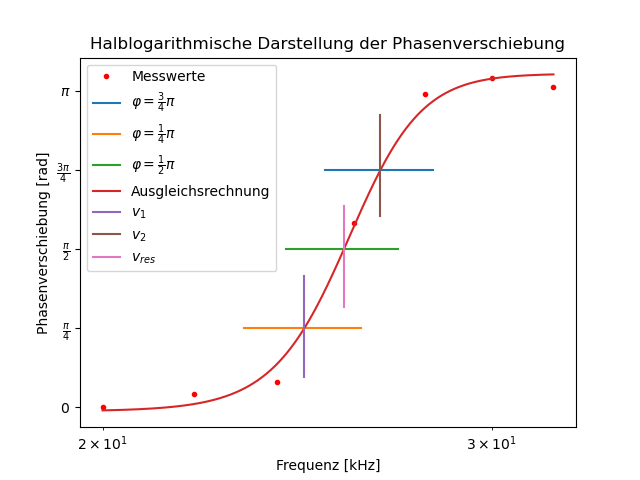
\includegraphics{5d.png}
\end{figure}

\noindent Für die benötigten Punkte sind nun die drei Schnittpunkte der eingezeichneten Waagerechten mit der Ausgleichskurve zu bestimmen.

\noindent Dafür wird die Formel der Ausgleichfunktion nach x umgestellt und die Parameter so wie die gegebenen Werte für die Phasenverschiebung werden eingesetzt.
Über den graphischen Ansatz ergeben sich also diese Werte:
\begin{center}
    \begin{tabular}{ll@{${}\pm{}$}l}
        \toprule
        Frequenz & Wert & Unsicherheit\\
        \midrule
        v\textsubscript{res} & 25.72 & 0.24     \\
        v\textsubscript{1} &  24.68 & 0.25      \\
        v\textsubscript{2} &  26.72 & 0.27      \\
        \bottomrule
        
    \end{tabular}
\end{center}

Die theoretischen Werte lassen sich mit den Folgenden zwei Formeln bestimmen:

\begin{align}
    \omega_{1,2} &= \pm \frac{R}{2L} + \sqrt{\frac{R^2}{4L^2}+\frac{1}{LC}} \nonumber\\
    \omega_{res} &= \sqrt{\frac{1}{L*C}-\frac{R^2}{4L^2}} \nonumber \\
\end{align}

\noindent Es ergeben sich mit den zu Beginn der Auswertung erwähnten Werte für C, L und R, wobie R\textsubscript{1} noch um 50 $\Omega$ vergrößert werden muss,
folgende Theoriewerte.:

\begin{center}
    \begin{tabular}{ll@{${}\pm{}$}l}
        \toprule
        Frequenz & Wert & Unsicherheit\\
        \midrule
        v\textsubscript{res} & 16.98 & 0.28     \\
        v\textsubscript{1} &  16.64 & 0.27      \\
        v\textsubscript{2} &  17.34 & 0.28      \\
        \bottomrule  
    \end{tabular}
\end{center}

\noindent Auch hier sind die auftretenden Abweichungen von den Theoriewerten mit ähnlichen Fehlerquellen behaftet.
Allerdings kommt hier noch erschwerend hinzu, dass die gemessenen Werte, 
bevor sie verwendet werden, 
schon in eine Rechnung involviert sind und sich der Fehler dort schon fortpflanzt.

\section{Diskussion}

Die Abweichungen der einzelnen Werte sind bei der jeweiligen Rechnung bereits diskutiert worden.
Es fällt jedoch auf, dass, obwohl viele verschiedene REchnungen durchgeführt werden, die Fehlerquellen relativ ähnlich bleiben.
Die Abweichung aller berechneten Werte lassen sich deutlich verbessen, wenn ein Gerät verwendet würde, 
welches eine genauere Möglichkeit bietet die Werte auch abzulesen. 
Das verwendete Gerät misst sehr genau und ist sehr empfindlich, jedoch ist das Ablesen der Werte aufgrund der Empfindlichkeit 
und der Beschaffenheit des Bildschirm nur verhältnismäßig grob möglich.
Eine digitale Anzeige der abzulesenden Werte wäre nicht nur einfacher sondern auch genauer.

\noindent Des Weiteren wurden viele Werte graphisch bestimmt.
Bei einer solchen Vorgehensweise werden immer bestimmte Ungenauigkeiten in Kauf genommen, 
da Ausgleichsrechnungen mit fehlerbehafteten größen zur weiteren Ungenauigkeiten führen.

\noindent Zusammenfassend lässt sich sagen, dass die experimentell bestimmten Werte zwar große,
aber keine unerklärbaren Abweichungen aufweisen.
Die zu zeigenden Zusammenhänge konnten auch gut mit diesen Werten dargestellt werden,
obwohl sie teilweise sehr weit von theoretischen Werten abweichen 
und deshalb ist das Ziel des Versuchs erreicht.


\section{Tabellen}

\begin{minipage}{\linewidth}
\begin{table}[H]
    \centering

\begin{tabular}{ll}
    \toprule
    Zeit [µs] & Spannung [V]\\
    \midrule
    0     & 4    \\   
    25    & 3.3  \\  
    50    & 2.8  \\  
    75    & 2.4  \\   
    90    & 2    \\   
    115   & 1.6  \\  
    140   & 1.4  \\   
    160   & 1.2  \\   
    185   & 1    \\   
    205   & 0.8  \\  
    225   & 0.7  \\  
    250   & 0.6  \\  
    270   & 0.5  \\  
    290   & 0.4  \\  
    315   & 0.35 \\   
    340   & 0.3  \\   
    \bottomrule
    
\end{tabular}
\captionof{table}{Spannungsamplituden}
\label{tab:5a}
\end{table}
\end{minipage}


\begin{minipage}{\linewidth}
    \begin{table}[H]
        \centering
    
    \begin{tabular}{ll}
        \toprule
        Frequenz [kHz] & $\frac{U_C}{U} [V]$\\
        \midrule
        5     & 1.08 \\
        10    & 1.24 \\
        15    & 1.44 \\
        20    & 2.16 \\
        21    & 2.40 \\
        23    & 3.00 \\
        24    & 3.40 \\
        25    & 3.72 \\
        26    & 3.80 \\
        27    & 3.64 \\
        28.5  & 3.12 \\
        30    & 2.44 \\
        33    & 1.60 \\ 
        35    & 1.24 \\
        40    & 0.84 \\
        45    & 0.60 \\
        50    & 0.44 \\ 
        \bottomrule
        
    \end{tabular}
    \captionof{table}{Resonanzfrequenz}
    \label{tab:5b}
    \end{table}
    \end{minipage}

    \begin{minipage}{\linewidth}
        \begin{table}[H]
            \centering
    \begin{tabular}{lll}
        \toprule
        Frequenz [kHz] & a [µs] & b [µs]\\
        \midrule
        20  &    0     &  32 \\
        22  &    0.6   &  28 \\
        24  &    1     &  25 \\
        26  &    7     &  24 \\
        28  &    10.4  &  21 \\
        30  &    10.4  &  20 \\
        32  &    9.6   &  19 \\ 
        \bottomrule
        
    \end{tabular}
    \captionof{table}{Phasenverschiebung}
    \label{tab:5d}
    \end{table}
\end{minipage}



\section{Quellen}

Versuchsanleitung zum Versuch 354 gedaempfte und erzwungene Schwingungen: \\
$https://moodle.tu-dortmund.de/pluginfile.php/1368604/mod_resource/content/1/V354.pdf$

\noindent Versuchsanleitung zum Versuch 353 Relaxationsverhalten eines RC-Kreises:\\
$https://moodle.tu-dortmund.de/pluginfile.php/1368601/mod_resource/content/1/V353.pdf$


\end{document}

